\documentclass[a4paper,10pt]{article}
\usepackage[utf8]{inputenc}
\usepackage{glossaries}
\usepackage{fullpage}
\usepackage{hyperref}
\usepackage{amsmath}
\usepackage{amsfonts}
\usepackage{graphicx}
\usepackage{subcaption}
\usepackage{verbatim}
\usepackage{pgfplots, pgfplotstable}
\usepackage{tikz}
\setlength\parindent{0pt}
\setlength{\parskip}{10pt}

\begin{document}
\begin{titlepage}

\newcommand{\HRule}{\rule{\linewidth}{0.5mm}} % Defines a new command for the horizontal lines, change thickness here

\center % Center everything on the page
 
%----------------------------------------------------------------------------------------
%	LOGO SECTION
%----------------------------------------------------------------------------------------

%----------------------------------------------------------------------------------------
 
%----------------------------------------------------------------------------------------
%	HEADING SECTIONS
%----------------------------------------------------------------------------------------

\textsc{\LARGE Progress report}\\
{\small NRF scarce skills 2014 and SKA NRF postgraduate funding 2015}\\
{\small Duration of funding: February 2014 - July 2015}\\[1.5cm]
%----------------------------------------------------------------------------------------
%	TITLE SECTION
%----------------------------------------------------------------------------------------

\HRule \\[0.4cm]
{ \huge \bfseries Bullseye: A parallel targeted facet imager}\\[0.4cm]
{ \large \url{https://www.github.com/ratt-ru/bullseye} (GNU GPL v3)}\\
\HRule \\[1.5cm]
 
%----------------------------------------------------------------------------------------
%	AUTHOR SECTION
%----------------------------------------------------------------------------------------

\begin{minipage}{0.4\textwidth}
\begin{flushleft} \large
\emph{Author:}\\
Benjamin \textsc{Hugo}\\[0.2cm] % Your name
\small{MSc. student}\\
\small{Department of Computer Science}\\
\small{University of Cape Town}\\
\small{bennahugo@aol.com}

\end{flushleft}
\end{minipage}
~
\begin{minipage}{0.4\textwidth}
\begin{flushright} \large
\emph{Supervisors:} \\
James \textsc{Gain} \\
Oleg \textsc{Smirnov} \\
Cyril \textsc{Tasse}\\
\end{flushright}
\end{minipage}\\[3cm]

% If you don't want a supervisor, uncomment the two lines below and remove the section above
%\Large \emph{Author:}\\
%John \textsc{Smith}\\[3cm] % Your name

%----------------------------------------------------------------------------------------
%	DATE SECTION
%----------------------------------------------------------------------------------------
{\large \today}\\[1.5cm] % Date, change the \today to a set date if you want to be precise
\vfill % Fill the rest of the page with whitespace

\end{titlepage}

\tableofcontents
\pagebreak
\listoffigures
\pagebreak
\section{Context}
There is a well-known fourier relationship between the coherence measurements taken with array-based radio telescopes and
the observed sky. Synthesis imaging entails creating an image of the sky through fourier inversion of these 
measurements between antenna pairs. The measurements are usually taken over extended periods of time, during which the 
directions between antennae with respect to a fixed point on the celestial sphere changes due to the rotation of the earth.
In effect multiple coherence measurements of the same source can be made in this way.

The computational complexity of directly inverting this relationship is roughly $\theta(N^4)$ using direct techniques, where
$N$ is the size in pixels of the sky image. To reduce this cost a Fast Fourier Transform may be used as a planar approximation
to the sky. However, this requires resampling the measurements onto a regularly-spaced grid. Furthermore, the planar 
approximation brakes down when imaging wider fields of view. This is illustrated in figure~\ref{FIG_WIDEFIELD_ERROR}.
\begin{figure}[h!]
  \centering
  \begin{subfigure}[b]{0.45\textwidth}
    \centering
    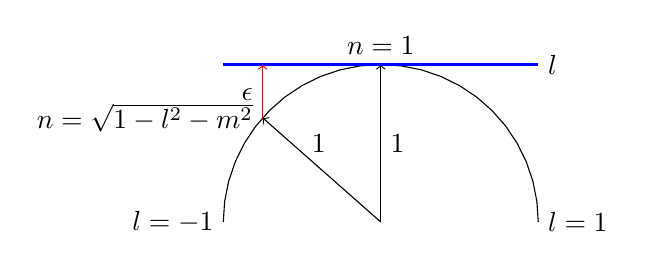
\begin{tikzpicture}
      \draw [black, domain=0:180] plot ({2*cos(\x)}, {2*sin(\x)});
      \draw [black, ->] (0,0) -- (0,2);
      \draw [black, ->] (0,0) -- ({-0.75*2},{sqrt(4-(-0.75*2)*(-0.75*2))});
      \node [above] at (0,1*2) {$n=1$};
      \node [right] at (0,0.5*2) {$1$};
      \node [right] at (-0.5*2,0.5*2) {$1$};
      \node [left] at ({-0.75*2},{sqrt(4-(-0.75*2)*(-0.75*2))}) {$n=\sqrt{1-l^2-m^2}$};
      \draw [blue,thick] (-2,2) -- (2,2);
      \draw [red, ->] ({-0.75*2},{sqrt(4-(-0.75*2)*(-0.75*2))}) -- ({-0.75*2},2);
      \node [left] at ({-0.75*2},{sqrt(4-(-0.75*2)*(-0.75*2))+0.15*2}) {$\epsilon$};
      \node [right] at ({1*2},{1*2}) {$l$};
      \node [right] at ({1*2},{0*2}) {$l=1$};
      \node [left] at ({-1*2},{0*2}) {$l=-1$};
    \end{tikzpicture}
    \caption{Error between the orthogonal planar FFT approximation to the sky and their actual positions on the celestial sphere}
  \end{subfigure}
  \begin{subfigure}[b]{0.45\textwidth}
    \centering
    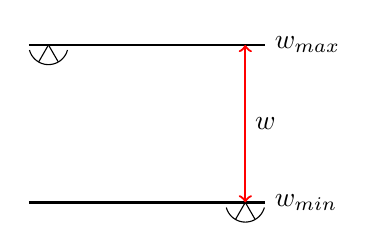
\begin{tikzpicture}
      \draw [black,thick] (0,2) -- (3,2);
      \draw [black,thick] (0,0) -- (3,0);
      \draw [black, domain={180+15}:{360-15}] plot ({(cos(\x)+1)*0.25}, {(sin(\x))*0.25+2});
      \draw [black] ({0.25*0.5},{2 - sqrt(0.25*0.25*(1-0.5*0.5))}) -- ({0.25},{2});
      \draw [black] ({0.25*1.5},{2 - sqrt(0.25*0.25*(1-0.5*0.5))}) -- ({0.25},{2});
      \draw [black, domain={180+15}:{360-15}] plot ({(cos(\x)-1)*0.25+3}, {(sin(\x))*0.25});
      \draw [black] ({3-0.25*0.5},{0 - sqrt(0.25*0.25*(1-0.5*0.5))}) -- ({3-0.25},{0});
      \draw [black] ({3-0.25*1.5},{0 - sqrt(0.25*0.25*(1-0.5*0.5))}) -- ({3-0.25},{0});
      \draw [red,thick,<->] ({3-0.25},{0}) -- ({3-0.25},{2});
      \node [right] at ({3-0.25},{1}) {$w$};
      \node [right] at ({3},{2}) {$w_{max}$};
      \node [right] at ({3},{0}) {$w_{min}$};
    \end{tikzpicture}
    \caption{Delay in signal propagation between antennas in an array-based telescope}
  \end{subfigure}
  \caption[Widefield phase delay]{The combined propagation delay of emission from sources far away from the telescope pointing centre is a combination
  of the error between the planar approximation and the celestial sphere in (a) and the delay difference between pairs of antennae in the telescope
  pointing direction as illustrated in (b). The total phase error is expressed as $w(n-1)$. The multiplicative effect of this w-term becomes a
  significant problem in large non-East-West antenna arrays, where the array components do not remain coplanar as the Earth rotates.}
  \label{FIG_WIDEFIELD_ERROR}
\end{figure}

The signal delay illustrated in figure~\ref{FIG_WIDEFIELD_ERROR} is manifested in the image as an apparent shift 
in source position. As measurements are integrated over hours of observation time this time-dependent shift leads to completely
smeared emission sources in the synthesized image. See figure~\ref{FIG_SMEARING}.
\begin{figure}[h!]
 \centering
 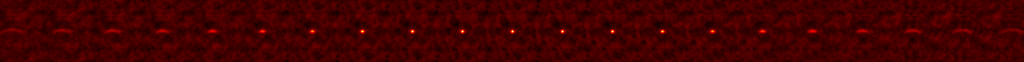
\includegraphics[width=0.9\textwidth]{images/distortions.png}
 \caption[Wide field distortions]{Sources further away from the telescope's pointing centre are smeared out over time, as
 shown in this simulated measurement.}
 \label{FIG_SMEARING}
\end{figure}

For narrow field images the resampling process only entails a convolution with an anti-aliasing filter that reduces energy of 
sources outside the field of view. This convolutional resampling and fourier inversion process has a cost of 
$\theta(N^2C^2) + \theta(N^2\log{N})$, where C is the support size of the convolution filter and is usually not much more 
than ten pixels per filter dimension.

When dealing with wide field images the cost of the resampling component quickly escalates to dominate the computational
complexity of the inversion process. There are 3 commonly used techniques to reduce the widefield smearing shown above:
\begin{enumerate}
 \item Faceting, where a wide field field of view is broken up into smaller narrow field images.
 \item W-projection, where the $w(n-1)$ term is convolved into the FFT relationship between the planar image and the emission sources
 on the celestial sphere.
 \item Snapshot imaging, where short duration images are made, reprojected and integrated into one final image.
\end{enumerate}

Since this costly resampling step will necessarily be called upon multiple times per observation for the purpose of deconvolving the 
effects of incomplete sampling, it is worth investigating how this step may be accelerated. Our work focuses on the convolutional 
resampling component of the first two approaches, a hybrid approach between faceting and W-projection. We focus on parallelizing
this hybrid faceting technique both using CPU multithreading techniques, as well as using General Purpose Graphics 
Processing Units.
\section{Facet imaging (2014)}
When performing facet imaging multiple smaller images of the sky are made. Each smaller image is made with respect to a new reference
centre, by phase shifting each coherence measurement. This effectively means that the resampling step has to be done for each
facet, and the computational complexity of the method grows with number of facets. The filter support region, however remains unchanged.

As Rick Perley \cite{perley1999imaging} points out it is also necessary to make the new facets tangent to the celestial sphere in order 
to keep the phase error over a fixed field of view comparable between facet images. Failure to do so will result in needing many
more facets towards the edge of a wide field image than in the centre. We've implemented this classic faceting approach in 2014 and obtained
good results with both simulated and calibrated data from the Extended Very Large Array. Our imager allows the user to either target the 
regions around a list of coordinates (figure~\ref{FIG_BULLSEYE}) or divide a continuous piece of sky into multiple facets.

\begin{figure}[h!]
 \centering
 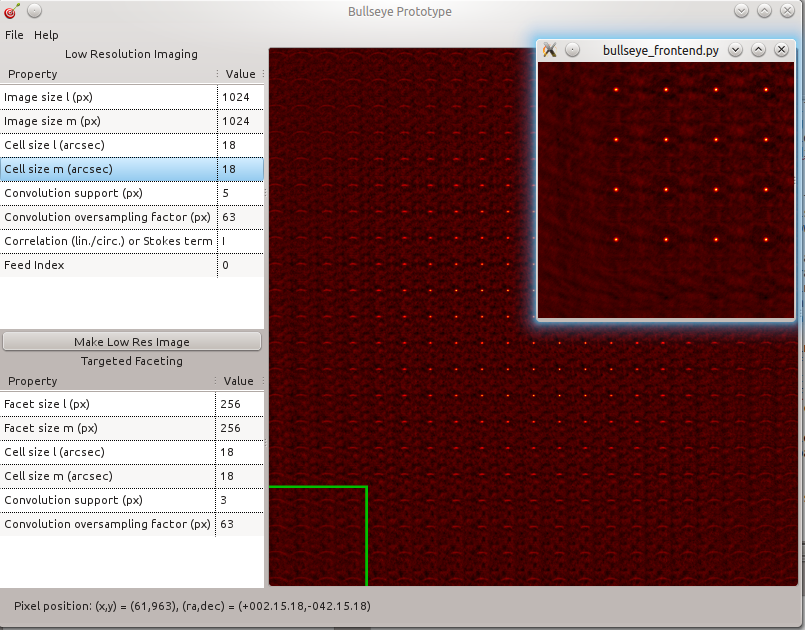
\includegraphics[width=0.75\textwidth]{images/targeted_faceting.png}
 \caption[Targeted faceting]{Here the prototype user interface for targeted faceting is demonstrated. A region towards the edge
 of a simulated grid sky model is faceted. The facet image is displayed in a new window.}
 \label{FIG_BULLSEYE}
\end{figure}

However, this approach poses a cumbersome problem. Since the facets are rotated through a rotation of the sampling coordinates, 
the Point Spread Function \footnote {Fourier transform of the sampling coordinates. Each source will be convolved with this function.
An example is the Gausian-like smearing around each point source in the simulated field in figure~\ref{FIG_SMEARING}. In this instance
the PSF is ideal. With other array configurations the PSF can take on more cumbersome forms} changes per facet. Unlike in normal 
narrow fieldimaging this effectively means that the PSF changes over the final image (each facet will have its own associated PSF). Thus, 
Because of this non-coplanar faceting complicates the task of deconvolution. 

We opted to investigate a coplanar faceting approach instead. With such an approach all the facet images are parallel to 
each other and can be jointly deconvolved. There are multiple ways to achieve coplanar faceting. Non-coplanar facets can be
re-projected and mosaiced onto a common plane using the transformations described by Sault et. al \cite{sault1996approach} in the measurement space 
or using existing mosaicing software, such as Montage \cite{jacob2004montage} in the image space. Doing the latter reprojection and 
background correction during every major deconvolution cycle can prove costly - both in the extra memory required and 
computation time.

Another approach that is more in line with the idea behind w-projection is to introduce an approximation of $w(n-1)$ while resampling.
Here Kogan and Greisen \footnote{AIPS Memo 113 (2009). Available from \url{http://www.aips.nrao.edu/aipsmemo.html}} uses a first order
tailor approximation to the error term, which we incorporated into our imager. A more accurate approach involves including a higher
order approximation to the error term through convolution as with w-projection. This increases the filter support size and the 
computational costs, but using such a hybrid approach it is possible to create larger facet images at the cost of slightly more
expensive gridding.
\section{Hybrid W-faceting (2015)}
In W-projection \cite{cornwell2008noncoplanar} the filtering operation in resampling is changed to include the error term. This filter has to be sampled
at a high enough rate to accomodate the rapidly changing w value at the edge of the image. The filter is precomputed for a
range of values for w between $w_{min}$ and $w_{max}$. While resampling the best-fit filter is picked depending on the
coordinate at which the coherence measurement is taken. See figure~\ref{FIG_W}.
\begin{figure}[h!]
 \centering
 \begin{subfigure}[b]{0.75\textwidth}
    \centering
    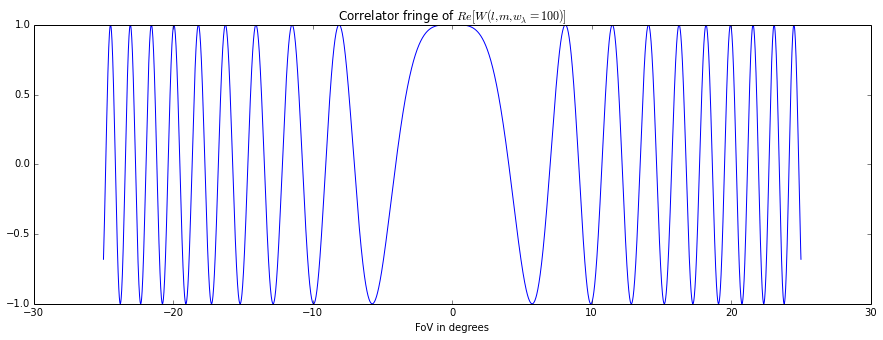
\includegraphics[width=0.75\textwidth]{images/w100.png}
 \end{subfigure}
 \begin{subfigure}[b]{0.75\textwidth}
    \centering
    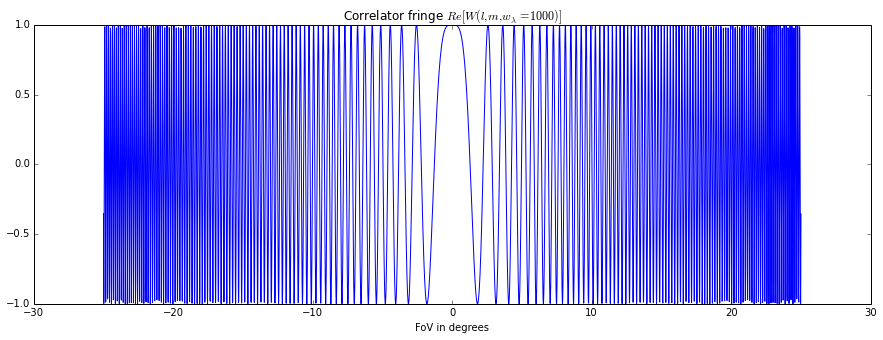
\includegraphics[width=0.75\textwidth]{images/w1000.png}
 \end{subfigure}
 \caption[W as a function of image size]{The W-term varies as a function of image size. Larger images have faster varying
 W-values at the edge of the image. This requires larger filters to accomodate this fast varying function. Non-East-West 
 Arrays with longer baselines have faster varying w values.}
 \label{FIG_W}
\end{figure}

With a hybrid approach \footnote{Suggested by the TDP Calibration group \cite{yashar2009tdp}} the facet images are smaller than those synthesized in a pure 
w-projection approach. The associated filter support regions, as well as number of w-values being computed, are also smaller. This 
makes the gridding operation more data parallel and less memory intensive than full w-projection - the latter requires careful consideration when creating 
images at the Nyquest rate required by the SKA layout (which may be up to $10^{10}$ pixels for the final image according to some estimates). 
Here either a faceting approach such as the one we're investigating may be needed or the gridding operation will have to be done in 
multiple passes.

Another advantage to combining faceting with w-projection is that, for smaller fields of view the filter becomes seperable, requiring far
less memory and precomputation time than its non-seperable counterpart. Additionally this filter is much more likely to fit into the cache memory
of General Purpose Graphics co-processors - this is essential to achieving good throughput on such architectures.
\section{Validation on observed EVLA data}
As part of our validation strategy we've selected a sample EVLA dataset. To ensure the usability of our imager
we support measurements stored in the NRAO Measurement Set format \footnote{NRAO CASA Memo 229. Available from \url{http://casa.nrao.edu/Memos/229.html}}.
The data we've selected as part of our standard set of test datasets is the calibrated and flagged measurement of the supernova
reminant G55.7+3.4 as observed using the EVLA D configuration at L-band. A continuium image is shown in Figure~\ref{FIG_SUPERNOVA}.
\begin{figure}[h!]
  \centering
 \begin{subfigure}[b]{0.49\textwidth}
    \centering
    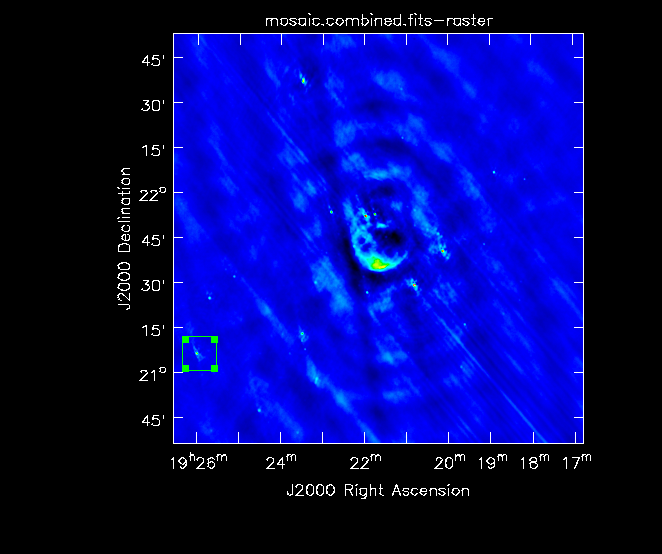
\includegraphics[width=\textwidth]{images/mosaic.png}
    \caption{Mosaiced faceted image (2x2 facets, 1.2\% padding). No additional w-projection.}
 \end{subfigure}
 \begin{subfigure}[b]{0.49\textwidth}
    \centering
    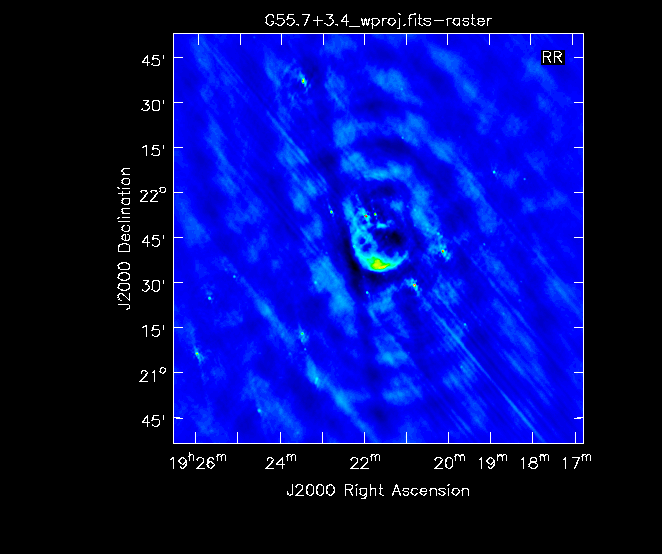
\includegraphics[width=\textwidth]{images/wproj.png}
    \caption{W-projected image. No faceting.}
 \end{subfigure}
 \begin{subfigure}[b]{0.49\textwidth}
    \centering
    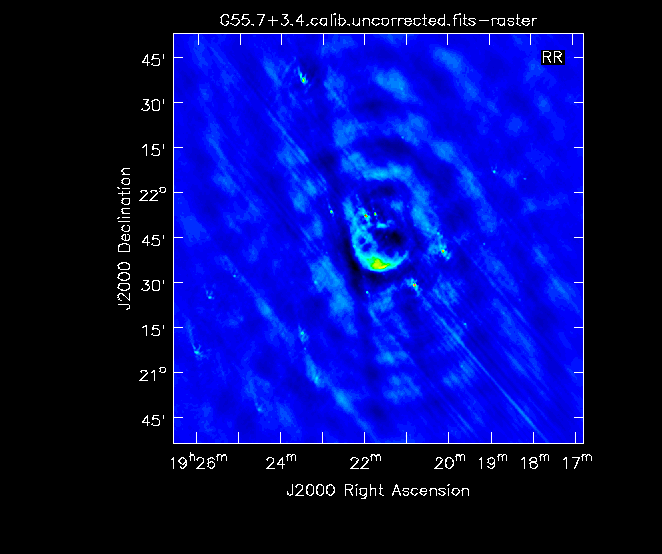
\includegraphics[width=\textwidth]{images/uncorrected.png}
    \caption{Uncorrected image (normal narrow field imaging).}
 \end{subfigure}
 \begin{subfigure}[b]{0.49\textwidth}
    \centering
    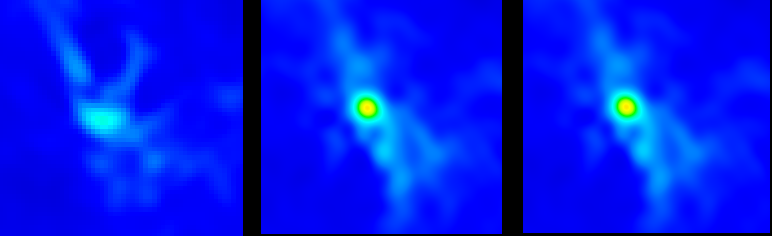
\includegraphics[width=\textwidth]{images/corrections.png}
    \caption{Up close, from the left: the uncorrected source, the faceted source and 
    finally the w-projected source}
 \end{subfigure}
 \caption[Supernova reminant G55.7+3.4]{In this field there is a clear widefield distorition near
 right assention $19h26m$, declination $21^\circ7'$. Both the faceting and w-projection
 implementations corrects the distortion as expected.}
 \label{FIG_SUPERNOVA}
\end{figure}
\section{Implementation progress}
\subsection{February 2014 - February 2015}
A significant portion of the code base for the imager was written during this period. This included a lock-based multithreaded 
CPU facet imager, based on the non-coplanar method discussed above. I additionally created a GPU-based implementation of the
convolutional resampling technique, based partly on a work distribution approach suggested by John Romein \cite{romein2012efficient}.
In this approach the correlation methods of each antenna pair is added to the regular grid in parallel. Because the tracks from these
antenna pairs are swept out slowly over the duration of an observation it is possible to limit global write operations, by accumulating
results in the register memory of the GPU. We further extended this approach to compute multiple facets in parallel. By the end of January 2015
the GPU-based implementation was working.
\subsection{March 2015 - June 2015}
Most of our effort during the past few months was focussed on adding coplanar faceting and rewriting most of the CPU convolutional resampling algorithm.
The approach we took focusses on a course-grained parallel approach to create facets in parallel, removing the need for locks. We further focussed on implementing
various forms of the w-projection algorithm and ensuring good performance on the CPU for the purpose of comparison. 

Because of the increased filter size a W-projection resampling approach is much slower than regular gridding. However, it does provide an opportunity
to better employ the vector instruction sets of modern CPUs. We've implemented w-projection employing AVX vectorization in addition to the course-grained 
parallelization achieved when creating multiple facets in parallel. This accounts for roughly 2 months worth of work.

During the few weeks I've also reworked a portion of my GPU resampling implementation to use seperable W-projection filters. The implementation now
caches the w-projection filters in a fast on-chip texture cache that limits accesses to global memory and ensures that the resampling time is roughly 20\% faster than
performing w-projection without this caching operation.
\subsection{Latest results}
I've included figures~\ref{FIG_RESULTS} to showcase our latest results. The modifications and improvements to the CPU-based resampling method
recently has made a dramatic improvement in runtime. This has made it comparable to a GPU based approach using Romeins distribution strategy,
as discussed earlier.

\begin{figure}[h!]
  \begin{subfigure}[b]{0.49\textwidth}
  \centering
   \resizebox{\linewidth}{!}{
      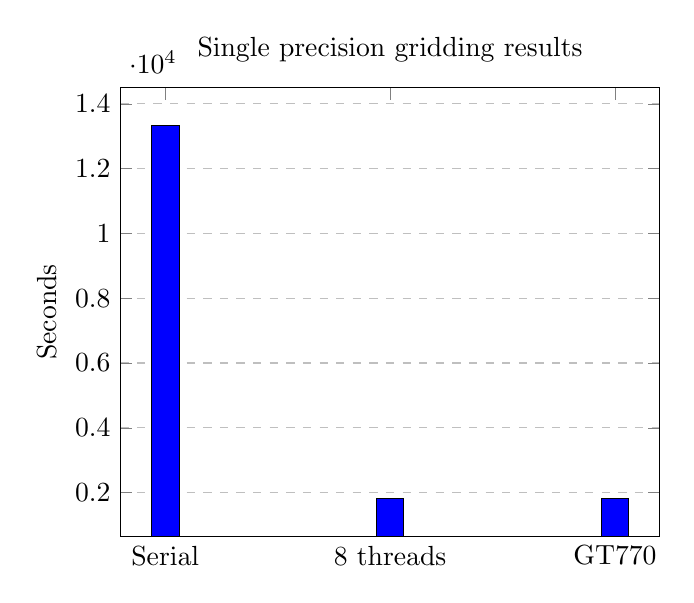
\begin{tikzpicture}
      \begin{axis}[
	  title={Single precision gridding results},
	  ylabel={Seconds},
	  ymajorgrids=true,
	  grid style=dashed,
	  symbolic x coords={Serial,8 threads,GT770},
	      xtick=data]
	      \addplot[ybar,fill=blue] coordinates {
		  (Serial,13342.452)
		  (8 threads,1823.442)
		  (GT770,1806.816)
	      };
      \end{axis}
      \end{tikzpicture}
  }
  \caption{Comparison between approaches using a hybrid 5x5 facets, w-projection with 31px support kernels}
  \end{subfigure}
  \begin{subfigure}[b]{0.49\textwidth}
    \centering
    \resizebox{\linewidth}{!}{
    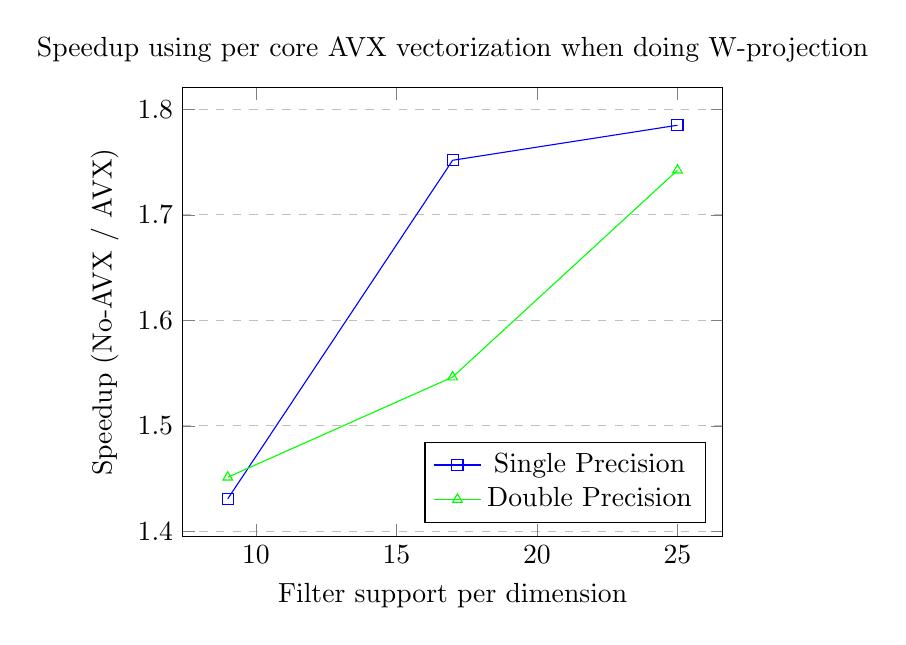
\begin{tikzpicture}
      \begin{axis}[
	  title={Speedup using per core AVX vectorization when doing W-projection},
	  xlabel={Filter support per dimension},
	  ylabel={Speedup (No-AVX / AVX)},
	  legend pos=south east,
	  ymajorgrids=true,
	  grid style=dashed,
      ]
      
      \addplot[
	  color=blue,
	  mark=square,
	  ]
	  coordinates {
	  (9,1.4308884327)(17,1.7517694033)(25,1.7849861029)
	  };
	  
      \addplot[
	  color=green,
	  mark=triangle,
	  ]
	  coordinates {
	  (9,1.4513690673)(17,1.5463198748)(25,1.7423449855)
	  };
	  \legend{Single Precision,Double Precision}
      \end{axis}
      \end{tikzpicture}
  }
  \caption{Speedup achieved per core when vectorizing the inner most loop in the resampling method using the AVX instruction set}  
  \end{subfigure}
  \caption[Acceleration Results]{The following results compares firstly the runtimes between sequential, CPU parallel and GPU parallel
    approaches (a) and secondly the performance impact of vectorizing w-projection resampling routines (b). Our latest optimizations
    on CPU-based facet resampling made it comparable to a GPU resampling implementation using Romein's work distribution strategy.
    In both plots the field G55.7+3.4 is being imaged. Our dataset has 778.91 MiB worth of correlation measurements (visibilities) 
    alone, excluding supporting data columns.}
  \label{FIG_RESULTS}
\end{figure}

\section{Work to be completed within the next few weeks}
Although the majority of the implementation agreed upon has been completed, there are still a few remaining smaller issues to be investigated and fixed. One of which is
the effect of doing the resampling in double precision instead of single precision. Support for this is already available in our imager, and the investigation simply entails
simulating several realistic fields and noting the effect of using double precision on the dynamic range of the images. There are also several small bug fixes and small 
optimizations that can still be made. This should not take more than 2 weeks to complete.

I aim to compare performance against other existing software packages and write up the relevant chapters on implementation and analysis during the 3rd and early 4th quarter
of the year and have my discertation ready for marking by December 2015. 
\section{Useful avenues of expansion considered out of scope in this project}
Our work primarily focussed on accelerating the convolutional resampling algorithm and constructing a viable imager to make dirty sky maps. However, there is significant
contributions to be made to the imager. One of which is adding a major-minor cycle deconvolution strategy. This should not prove to be too difficult since
the coplanar facet images can be jointly deconvolved.

Additionally facet imaging provides an opportunity to deal with Directional Dependent Effects. One of the most crutial is the removal of the effects introduced by the antenna
response pattern. In previous years antenna beam pattern models only consisted of overly simplistics analytic functions. However, improved antenna sensitivity in recent upgrades to
existing and new telescopes has warented a refreshed look at older calibration and correction techniques. Correcting for the antenna beam pattern in the imaging step will prove very
useful in widefield imaging, where sources may lay outside the primary beam of the telescope. Using facet imaging to approximate the beam pattern while resampling is certainly a promising
way of dealing with the new reality. Bullseye already has some functionality to read time and frequency varient matricies from an extended measurement set format and all that remains is to
propagate those tables with values derived from a realistic beam pattern model.

It should be noted that Bullseye is intended to be used as a continuium imager. A useful addition will be the incorporation of 
relativistic effects necessary to do spectral imaging in very narrow bands.
\pagebreak
\bibliography{ska_progress_report}{}
\bibliographystyle{plain}
\end{document}          
